\section{Agregar Tratamiento}

Cuando un paciente se enferma y recurre a visitar al doctor, éste le dará un nuevo tratamiento, con nuevas instrucciones y medicamentos, entonces de esta manera el usuario podrá agregar un tratamiento nuevo en donde establecerá cuantos medicamentos tiene que tomar, cuándo se expidió el tratamiento y quién es el doctor encargado de este.

\subsubsection{Procedimiento}
\begin{enumerate}
	
	\item Da clic en el botón \textbf{Agregar Paciente} de la pantalla \textbf{Pacientes}.
	
	\item Se mostrará la pantalla \textbf{Agregar Paciente}.
	\newpage
	\begin{figure}[!htbp]			
		\hypertarget{fig:AgregarPaciente}{\hspace{1pt}}
		\begin{center}
			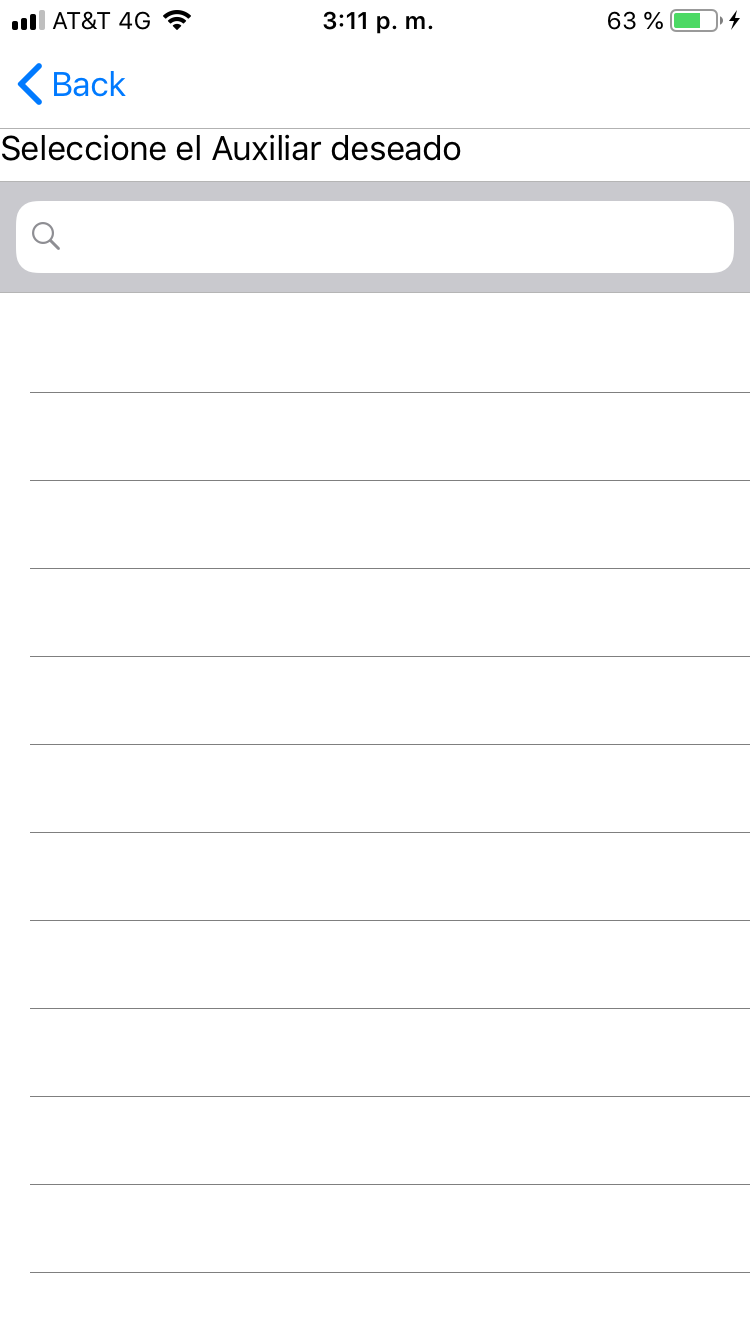
\includegraphics[height=0.4\textheight]{Paciente/AgregarAuxiliar/images/AgregarAuxiliar}
			\caption{Agregar Paciente}
			\label{fig:AgregarPaciente}
		\end{center}
	\end{figure}
	
	
	\item Ingrese el paciente deseado y seleccione la opción Desea agregar un tratamiento al paciente.
	
	\item Se mostrará la pantalla \textbf{Agregar Nuevo Tratamiento}
	\newpage
	\begin{figure}[!htbp]			
		\hypertarget{fig:AgregarTratamiento}{\hspace{1pt}}
		\begin{center}
			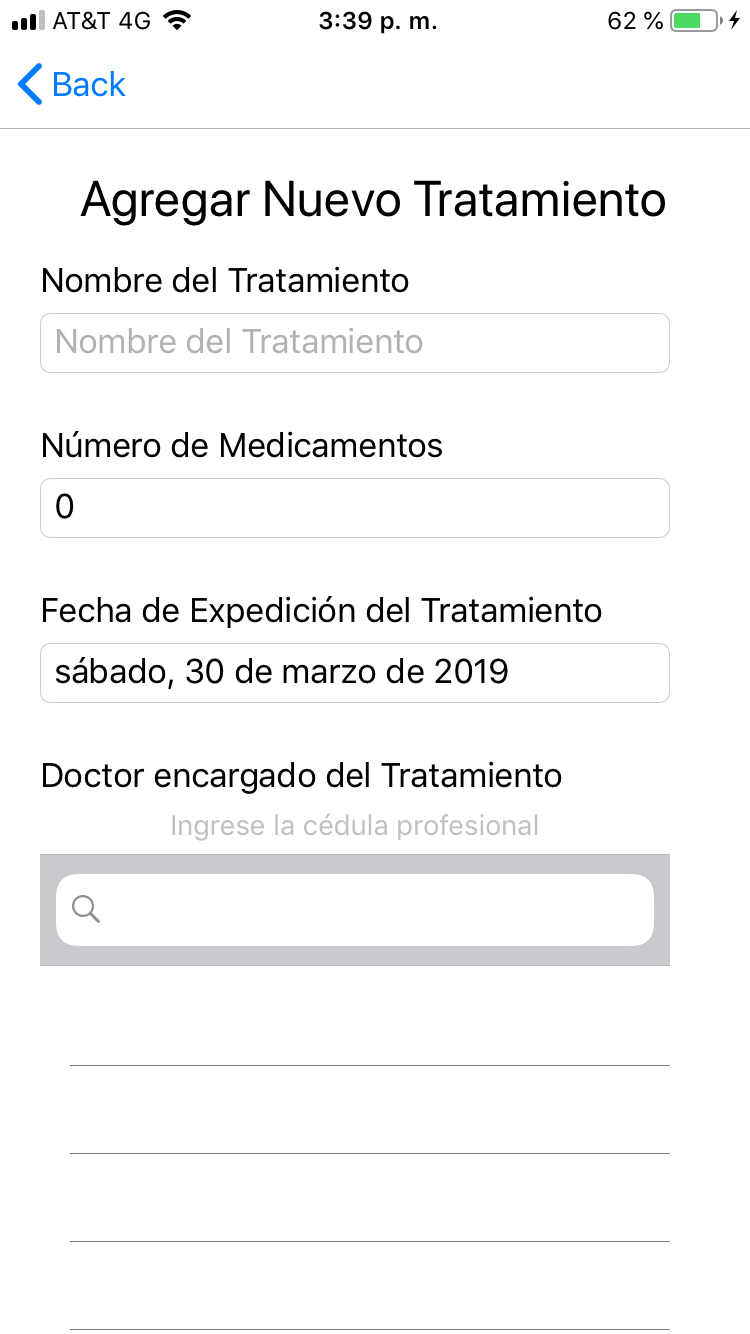
\includegraphics[height=0.4\textheight]{Paciente/AgregarTratamiento/images/AgregarTratamiento}
			\caption{Agregar Nuevo Tratamiento}
			\label{fig:AgregarTratamiento}
		\end{center}
	\end{figure}
	
	\item Ingresa los datos solicitados por la pantalla \textbf{Agregar Nuevo Tratamiento}
	
	\item Presiona el botón \textbf{Agregar}.
	
\end{enumerate}

